\subsection{World state generation}

The world states under consideration in this task are referred to as ``contexts''. Each context comprises a sequence of randomly chosen cuisenaire rods, each of which has a given colour (chosen from a set of 8) and length (ranging from 1-10). A context can have up to 13 rods, and from the context a random subset is selected.

The goal of the task is to write an utterance which correctly identifies the selected rods from among the rest in the context. This problem was constructed to be similar to a typical first language lesson according to the Te Ataarangi method.

Sampling uniformly from a large world state space would result in a large proportion of states with high entropy. This would be undesirable, since the goal is to teach the language so we chose to start from simpler world states and gradually increase the complexity. For that reason, we used the following procedure to generate arrangements of cuisenaire rods:

\begin{itemize}
\item An entropy budget is chosen, calculated as the sum of the entropy for colour and height.
\item A rod is selected with random height and colour, and the entropy for the new configuration is computed.
\item If this entropy exceeds the threshold, the process ends; otherwise, another rod is added.
\end{itemize}

\subsection{Labelling world states}

During labelling, the entropy budget begins set to 0.5, and then every 66 examples the budget was increased by 0.5 to a cap of 8.0 resulting in a sample size of 990. For certain easy cases, such as when all rods are selected, a pre-computed utterance such as ``ngā rākau katoa'' (``all of the rods'') or ``te rākau'' (``the rod'') would automatically be entered on behalf of the user. This happened in approximately 30\% of the examples in the dataset.

\subsection{Conversational Agents}

In this work, we aim to implement a pair of conversational agents. A teacher $A_{teacher}$, and a student $A_{student}$. The agents comprise of two models, the first maps contexts to utterances. In the case of the teacher, this model is pre-trained to be correct, while the student begins with a randomly initialised model.

The second model is designed to suggest world states for demonstration. For the teacher, this functions as a curriculum that takes in the history of (context, utterance) pairs from the student, and suggests world states that will help the student arrive at correct conclusions. In the case of the student, the world states are chosen to demonstrate that it has acquired the ability to produce correct utterances for the kinds of world states that the teacher has demonstrated so far, as well as to make conjectures that will demonstrate that the patterns it has learned generalise in the right way.

\subsection{The dataset}

In order to learn this task, we prepared a dataset of (context, utterance) pairs. The dataset consists of 1,017 such pairs, where each world state is represented as a list of rod objects each with colour, height and an additional true/false value indicating whether it has been selected or not. The world states were rendered as images, and then labelled with the utterance.

\begin{table}[h]
  \centering
  \begin{tabular}{|p{3cm}|p{3cm}|}
    \hline
    te reo Māori & English translation \\ \hline
    Ngā rākau katoa & All of the rod \\ \hline
    Te rākau         & The rod (singular)  \\ \hline
    Te rākau iti     & The small rod  \\ \hline
    Te rākau whero   & The red rod  \\ \hline
    Te rākau whero me te rākau iti rawa & The red rod and the smallest one \\ \hline
  \end{tabular}
  \caption{Example utterances from the dataset}
  \label{tab:example_table}
\end{table}

The utterances for all of the (context, utterance) pairs are written using only 29 unique tokens.

\begin{figure}[htbp]
  \centering
  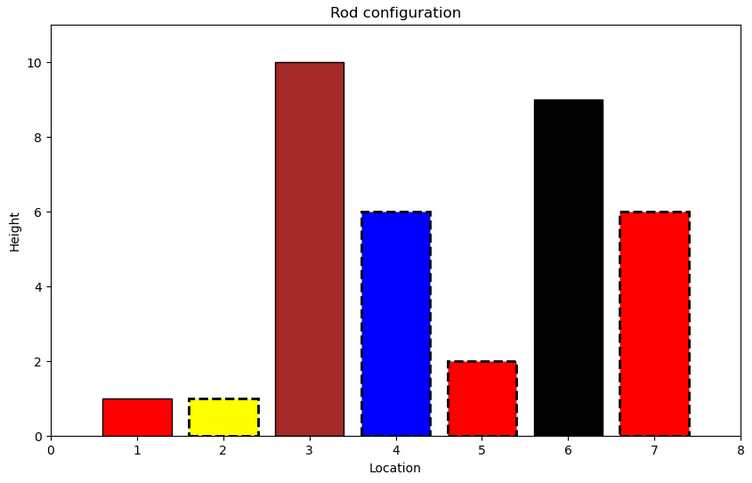
\includegraphics[width=0.4\textwidth]{images/rākau_plot.png} % Adjust the path and image file name
  \caption{An example arrangement of rods. The utterance for this configuration is: ``te rākau kōwhai me te rākau kikorangi me ngā rākau whero katoa hāunga te rākau iti rawa''/''The yellow rod, and the blue rod, and all of the red rods except for the smallest one``. Note that the selection is given by dotted-lines.}
  \label{fig:rākau_plot} % Label for referencing the figure in text
\end{figure}

\subsection{Tokenisation}

Each context was converted to a sequence of tokens so that the labelling problem could be approached as a translation task. The complete list of context tokens are given in table \ref{tab:state_tokens}. The tokens are then arranged in the order \texttt{[SOS]}, then whether the current rod is selected (\texttt{[SELECTED]/[NOT\_SELECTED]}) then its colour (e.g. \texttt{[COLOUR\_RED]}), followed by its height (e.g. \texttt{[HEIGHT\_3]}). Subsequent rods are then appended to this sequence according to the same rule (selection, colour, height), and the last state token is followed by the \texttt{[SEP]} token.

\begin{table*}[t]
\centering
\begin{tabular}{|>{\ttfamily}l|p{12cm}|}
\hline
\textbf{Token}         & \textbf{Description} \\ \hline
[PAD]                  & Padding token used to fill empty spaces in data sequences to ensure uniform length. \\ \hline
[SOS]                  & Start of sequence token, used to signal the beginning of a new data sequence. \\ \hline
[SELECTED]             & Token indicating that an item or feature is selected or active in the context. \\ \hline
[NOT\_SELECTED]        & Token indicating that an item or feature is not selected or inactive in the context. \\ \hline
[COLOURS]              & Tokens representing various colors (red, blue, green, yellow, black, white, brown, pink). \\ \hline
[HEIGHTS]              & Tokens representing various height levels (1 to 10). \\ \hline
[SEP]                  & Separator token. \\ \hline
\end{tabular}
\caption{Context state tokens with descriptions}
\label{tab:state_tokens}
\end{table*}

The utterances were tokenised simply as regular words, and the complete token list is included in the appendix.

\subsection{Data augmentation}

With such a small dataset, it would be challenging to learn a mapping even with a simple model. For this reason, we used data augmentation to increase the size of the dataset one thousand-fold. This was done by exploiting the following properties of the simple world-model.

\begin{itemize}
\item If you permute the colours in the context and the utterance in the same way, the resulting pair is still valid.
\item Unless the utterance mentions something location-specific (such as 'left'/'right') then the order of the rods can be permuted.
\item If 'left'/'right' are mentioned, then if you reverse the order of the rods then you can flip 'left'/'right' in the utterance.
\item In the utterances, the height of each rod was used only as an ordinal variable. Therefore any re-scaling of the rod heights which preserves order is consistent with the original utterance.
\end{itemize}

There are some limitations to this approach. In particular, permuting the rods randomly in this manner could result in an arrangement where some other utterance would more naturally occur to a human. For example, if the selected rods are all put on one side of the arrangement, then it may not be necessary to individually name specify each rod.

For the sake of keeping the problem simple, while growing the dataset enough that a model would be able to learn the pattern we went ahead with this approach.

\subsection{one-gram model}

To try and help the model learn with less human-labelled data we also used the labelled data to construct a one-gram model, which was used to constrain the output of the model by penalising the model for predicting any (previous, next) token pair that is not in the training data.

Since it is possible the coverage of all of the important token-pairs in the training set was not complete, each token in the dataset was assigned a part of speech class. Then the next-token restriction was applied based on token classes rather than individual tokens. This way words that have equivalent functions are treated equally by the one-gram model, and in case the training data did not cover a particular case (e.g. ``te rākau iti whero kei te taha mauī''/``the small red stick on the left'') we can still ensure that the model is aware that it's a valid utterance in principle. This does not prevent many other kinds of errors, such as infinite repetition using conjunction.

In order to penalise the model, the logits for any next-tokens that are not valid according to the one-gram model were set to a large negative value. The class labels assigned to each token, as well as the next-token classes map are provided in the appendix.

\subsection{Models}

The goal task was framed as translation, where the input sequence was the tokenised representation of the context, and the target sequence to be predicted is the utterance corresponding to that state. Therefore we approached this problem using sequence-to-sequence models.

We tried three model architectures, transformer, vanilla RNN and LSTM. Parameter sweeps were conducted to find hyperparameters for each.
